\def\year{2018}\relax
%File: formatting-instruction.tex
\documentclass[letterpaper]{article} %DO NOT CHANGE THIS
\usepackage{aaai18}  %Required
\usepackage{times}  %Required
\usepackage{helvet}  %Required
\usepackage{courier}  %Required
\usepackage{url}  %Required
\usepackage{graphicx}  %Required
\frenchspacing  %Required
\setlength{\pdfpagewidth}{8.5in}  %Required
\setlength{\pdfpageheight}{11in}  %Required
\usepackage{bm}
\usepackage{amsmath}
\usepackage{arydshln}
\usepackage{amsfonts}
\usepackage[ruled,vlined]{algorithm2e}
\usepackage{setspace}
\SetKwComment{Comment}{$\triangleright$\ }{}
\usepackage{caption}
\usepackage{subcaption}
\usepackage{float}
\usepackage{setspace}
\usepackage{amsthm}
\usepackage{multirow}
\usepackage{footnote}
\makesavenoteenv{tabular} \makesavenoteenv{table}
\usepackage{caption}
\usepackage{subcaption}
\usepackage{enumitem}
\newtheorem{theorem}{Theorem}
\newtheorem{definition}[section]{Definition}
\newtheorem{proposition}[theorem]{Proposition}
\usepackage{color}
\usepackage{mwe}
\usepackage{bbm}
\usepackage{epstopdf}


\ifodd 1
%\newcommand{\rev2}[1]{{\color{blue}#1}}%revise of the text
\newcommand{\rev}[1]{#1}
\newcommand{\frev}[1]{{\color{magenta}#1}}%revise of the text
\newcommand{\com}[1]{\textbf{\color{red}(COMMENT: #1)}} %comment of the text
\newcommand{\clar}[1]{\textbf{\color{green}(NEED CLARIFICATION: #1)}}
\newcommand{\response}[1]{\textbf{\color{magenta}(RESPONSE: #1)}} %response to comment
\else
\newcommand{\rev}[1]{#1}
\newcommand{\frev}[1]{#1}
\newcommand{\com}[1]{}
\newcommand{\clar}[1]{}
\newcommand{\response}[1]{}
\fi

%PDF Info Is Required:
  \pdfinfo{
/Title (A Reinforcement Learning Framework for Eliciting High Quality Information)
/Author (Zehong Hu,  Liu, Yitao Liang and Jie Zhang)} 
\setcounter{secnumdepth}{0}
 \begin{document}
% The file aaai.sty is the style file for AAAI Press 
% proceedings, working notes, and technical reports.
%
\title{A Reinforcement Learning Framework for Eliciting High Quality Information}
\author{Zehong Hu\textsuperscript{1,2}, Yang Liu\textsuperscript{3}, Yitao Liang\textsuperscript{4} and Jie Zhang\textsuperscript{2}\\
1 Rolls-Royce@NTU Corporate Lab, Nanyang Technological University, Singapore\\
2 School of Computer Science and Engineering, Nanyang Technological University, Singapore \\
3 Harvard University, USA\\
4 University of California, Los Angeles, USA\\}
\maketitle
\begin{abstract}
Peer prediction is a class of mechanisms that help elicit high-quality information from strategic human agents when there is no ground-truth for verifying contributions. Despite its elegant design, peer prediction mechanisms often fail in practice, mostly due to two shortcomings: (1) agents' incentives for exerting effort to produce high-quality information are assumed to be known; (2) agents are modeled as being fully rational. In this paper, we propose the first reinforcement learning (RL) framework in this domain, \emph{Reinforcement Peer Prediction}, to tackle these two limitations. In our framework, we develop a RL algorithm for the data requester to dynamically adjust the scaling level to maximize his revenue, and to pay workers using peer prediction scoring functions. Experiments show significant improvement in data requestor's revenue under different agent models.
\end{abstract}

\section{Introduction}
Crowdsourcing rises as a promising inexpensive method to collect a large amount of training data quickly \cite{snow2008cheap,deng2009imagenet}.
Notwithstanding its high efficiency, one salient concern about crowdsourcing is the quality of the collected information, as it is often too costly to verify workers' contributions.
This problem is called information elicitation without verification~\cite{waggoner2014output}.
A class of incentive mechanisms, collectively called peer prediction, has been developed to solve this problem~\cite{miller2005eliciting,jurca2009mechanisms,witkowski2012robust,witkowski2012peer,radanovic2013robust}.
The core idea of peer prediction is quite simple and elegant -- the mechanism designer financially incentivizes
workers according to the scoring of their contributions in comparison with their peers'. The payment rules are designed so that each worker reporting truthfully or reporting a high-quality signal is a strict Bayesian Nash Equilibrium for all workers.

Many peer prediction mechanisms adopt the effort-sensitive model to depict agents' trade-off reasoning in contributing high-quality information~\cite{witkowski2013dwelling,dasgupta2013crowdsourced,shnayder2016informed,liu2017sequential}. In these mechanisms, workers are incentivized to exert high effort to generate high-quality answers.
One critical assumption in those mechanisms is an explicitly-known worker model which includes workers' incentives. Furthermore it is also assumed workers are fully rational, following the utility-maximizing strategy. Unfortunately, neither is true in practice. Firstly, workers' incentives %, or cost,%
to exert high effort can most likely only be known after we, as the mechanism designers, interact with them. Secondly, there is strong evidence showing that human workers are not fully rational, and they are often observed to be deviating from equilibrium strategies in practice \cite{mckelvey1995quantal,jurca2007robust,gao2014trick}. Note \cite{gao2014trick} explicitly pointed this issue out in the peer prediction setting. 

To push peer prediction mechanisms towards being more practical, we propose a reinforcement learning (RL) framework, \emph{Reinforcement Peer Prediction}, to interact with workers, so as to (1) incentivize workers to converge to a high effort exertion state, and (2) learn the optimal payment based on workers' contributions at each step.
Nevertheless, we face two main challenges.
Firstly, classic reinforcement learning focuses on the interaction between a single agent and its environment. We, instead, need to effectively consider a multi-agent setting. Immediately more convoluted state evolution processes are formed among workers, because our incentive strategy relies on the comparison between workers' answers and their peers'. Specifically, the evolution of workers' state is a outcome of collective actions from all workers, as well as the environment. Secondly, no ground-truth is available to evaluate either the state of the workers or the rewards in our setting, whereas it is taken as granted in most other reinforcement learning frameworks. Due to these two challenges, until a proper way to evaluate workers' contributions is proposed, no model-free RL algorithms which learn from reward signals can be applied.
%Hence, we need to find a proper way to evaluate workers' contributions so that model-free RL algorithms which learn based on the reward signal can be applied.

Integrating both fields, reinforcement learning and peer prediction, we could successfully use one's advantage to resolve the other's limitation, and as a whole an approach appealing to a broader interest potentially emerges. More specifically,  the main contributions of this paper are as follows.
(1) We propose the first reinforcement peer prediction mechanism which does not need to assume a decision-making model for workers and the uninformative equilibrium where agents report uninformative information is a bad equilibrium.
Our mechanism combines a peer prediction mechanism with reinforcement learning to jointly incentivize workers and learn the optimal scaling level at each step.
(2) Due to the lack of ground-truth, we adopt Bayesian inference to evaluate workers' contributions, and to infer the reward following each action (i.e. offered scaling level). We derive the explicit posterior distribution of workers' contributions and employ Gibbs sampling to eliminate its bias.
(3) In our setting, the inferred contributions are corrupted by noise and only the most recent previous state rather than the current can be observed. We use the online Gaussian process regression to learn the $Q$-function and replace the unknown current state with the pair of the last observed state and scaling level (action).
(4) We conduct empirical evaluation, and the results show that our mechanism is robust, and is able to significantly increase data requester's revenue under different worker models, such as fully rational, bounded rational and learning agent models.

\section{Problem Formulation}
Our proposed mechanism mainly works in the setting where one data requester, at every step, assigns $M$ binary tasks with answer space $\left\{1,2\right\}$ to $N \geq 4$ candidate workers. At step $t$, worker $i$'s labels for the task $j$ is denoted as $L_i^t(j)$, and correspondingly the payment that the data requester pays is denoted as $P^{t}_i(j)$. Note we use $L^{t}_i(j)=0$ to denote task $j$ is not assigned to worker $i$ at step $t$, and naturally under this case $P^{t}_i(j)=0$.
After every step, the data requester collects labels and aggregates them through Bayesian inference~\cite{zheng2017truth}.
Denote the aggregated labels as $\hat{L}^{t}(j)$, and we can compute the accuracy as $A_t = \frac{1}{M}{\sum}_{j=1}^{M} 1(\hat{L}^{t}(j) = L^{t}(j))$.
The revenue for the data requester can then be computed as
\begin{equation}
r_t = F(A_t) - \eta {\sum}_{i=1}^{N}{\sum}_{j=1}^{M}P^t_i(j)
\end{equation}
where $F(\cdot)$ is a non-decreasing monotonic function mapping accuracy to revenue and $\eta$ is a
tunable parameter balancing label quality and costs. Intuitively, the $F(\cdot)$ function needs to be non-deceasing as higher accuracy is preferred and also labels are only useful when their accuracy reaches a certain requirement. Note our framework is robust to any formulation of $F(\cdot)$ function. If not otherwise specified, $F(\cdot)$ is set as $F(A_t)=A^{10}_t$ in our experiments.
Our goal is to maximize the cumulative discounted revenue $R = \sum_{t=1}^{T} \gamma^{(t-1)} r_t$, where $\gamma\approx 1.0$ is the discount rate and $T$ is the ending time, by making wise choices of actions  (i.e. deciding the offered scaling levels) at each step.

\section{Reinforcement Peer Prediction}
We present \emph{Reinforcement Peer Prediction} in Figure~\ref{ED1}. Note at every step $t$, the payment to worker $i$ for task $j$ is factored as a function over two elements, namely $P^{t}_i(j)=I_t \cdot p^{t}_i(j)$, where $I_t\geq 0$ is the scaling level decided by our RL algorithm, and
$p^t_i(j)$ is the output of our peer prediction scoring function.
Here, we assume that the available scaling levels are limited and they form a set $W$.
Thus, the action space of our RL algorithm is $W$ and it needs to learn the optimal policy to adjust the scaling level $I_t\in W$ so that the data requester's revenue $R$ can be maximized.

Since the ground-truth is not available, we cannot directly compute the reward (i.e accuracy $A_t$), following each action (i.e. deciding the offered scaling level).
Following MAP (maximum a posteriori estimation) principle, we resort to the expected value $\mathbb{E}A_t$ as an unbiased estimator of the real accuracy $A_t$.
It can be calculated as
\begin{equation}
\mathbb{E}A_t = \frac{1}{M}{\sum}_{j=1}^{M} \textrm{Pr}(\hat{L}^{t}(j) = L^{t}(j))
\end{equation}
where $\hat{L}^{t}(j)$s and $L^{t}(j)$s are the aggregate and true labels at step $t$, respectively. Besides used to aggregate data, Bayesian inference is also used to generate confusion matrices of all workers and the distribution of task labels $\left[\textrm{Pr}(L =1), \textrm{Pr}(L=2)\right]$, with again $L$ denoting the ground-truth label.


For worker $i$, his confusion matrix $C_i = [c_{ikg}]_{2\times 2}$ is a measurement of how much effort he exerts, where $c_{ikg}$ denotes the probability that worker $i$ labels a task in class $k$ as class $g$. Each worker can chose to exert either High effort or Low effort. Denote this decision variable as $e_i$. Exerting high effort leads a more accurate confusion matrix (higher values on diagonal), but it will also incur a cost $b>0$. 

Since the accuracy of labels is determined by the overall effort of workers, we denote the state of the whole worker crowd $s_t$ by workers' average probability of being correct, namely
\begin{equation}
s_t =\frac{1}{N}\cdot {\sum}_{k=1}^2\textrm{Pr}(L=k)\cdot  {\sum}_{i=1}^{N}c_{ikk}.
\end{equation}
After receiving the payment, workers may potentially adjust their strategies in exerting effort based on their rationality model, leading to the change of their state $s_t$.
However, when deciding the next-step scaling level $I_{t+1}$, we can only estimate the last step state $s_t$.
In other words, the state observation in our mechanism is not only imperfect, but also one-step delayed. This also makes our reinforcement learning problem different from traditional ones.
\begin{figure}[!htb]
        \includegraphics[width=0.5\textwidth]{image/Mechanism}
        \caption{\label{ED1} Illustration of our mechanism}
\end{figure}


\subsection{Peer Prediction Mechanism} 

We adopt the multi-task mechanism proposed by Dasgupta and Ghosh \shortcite{dasgupta2013crowdsourced}.  For each worker-task pair $(i, j)$, it selects a reference worker $k$. Suppose workers $i$ and $k$ have been assigned $d$ other distinct tasks $\{i_1,\ldots,i_d\}$ and $\{k_1,\ldots, k_d\}$, respectively. Then, the payment to worker $i$ after he labels task $j$ as $L^t_i(j)$ computes as
\begin{equation}
p^t_{i}(j)= \mathbbm{1}[L^{t}_i(j)=L^{t}_k(j)]- \xi_{i}^d\cdot \xi_{k}^d -\bar{\xi}_{i}^d\cdot \bar{\xi}_{k}^d
\end{equation}
where $\xi_{i}^{d}=\sum_{g=1}^{d}\mathbbm{1}(L^{t}_k(i_g)=1)/d$ and $\bar{\xi}_{i}^{d}=1-\xi_{i}^{d}$. 

We adopt above specific mechanism mainly for two reasons. First is due to its simple and prior-free implementation. Second is due to the fact that uninformative equilibrium where agents all report the same labels is a bad equilibrium under this mechanism.


\subsection{Bayesian Inference} Suppose the prior distributions follow: $$c_{ik1}\sim \textrm{Beta}(\alpha^{p}_{ik1},\alpha^{p}_{ik2})$$ and $$\textrm{Pr}(L=1)\sim \textrm{Beta}(\beta^{p}_{1},\beta^{p}_{2})$$ Then, we can explicitly derive the posterior distribution of the true labels of the assigned tasks, using the collected labels from workers, as follows:
\begin{align}
&\textrm{Pr}\left(L^{t}(1),\ldots, L^{t}(M)|\mathcal{L}^{t}\right)\propto B(\bm{\beta}^{t}){\prod}_{i=1}^{N}{\prod}_{k=1}^{K} B(\bm{\alpha}^{t}_{ik}) \nonumber \\
&\alpha^{t}_{ikg}={\sum}_{j=1}^{M}\delta^{t}_{ijg}\xi^{t}_{jk}+\alpha^{p}_{ikg}, \beta^{t}_k={\sum}_{j=1}^{M}\xi^{t}_{jk}+\beta^{p}_{k} \label{PostDist}
\end{align}
where $\mathcal{L}^{t}$ denotes the set of all collected labels and $B(\cdot)$ denotes the beta function, $\delta^{t}_{ijg}=\mathbbm{1}(L^t_i(j)=g)$ and $\xi^{t}_{jk}= \mathbbm{1}(L^{t}(j)=k)$. According to Gibbs sampling, we can generate posterior samples via iteratively sampling the following conditional probability distribution
\begin{equation}
\begin{split}
&\textrm{Pr}\left(L^{t}(j)|\mathcal{L}^{t},L^t (s\neq j)\right)\propto\\ &\qquad\qquad\qquad\textrm{Pr}\left(L^{t}(1),\ldots, L^{t}(M)|\mathcal{L}^{t}\right).
\end{split}
\end{equation}
After generating $W$ posterior samples
\begin{equation*}
\{(L^{t(1)}(1),\ldots, L^{t(1)}(M)),\ldots, (L^{t(1)}(1),\ldots, L^{t(1)}(M))\},
\end{equation*}
we can calculate the posterior distribution estimation for the true label of task $j$ as
\begin{equation}
\textrm{Pr}\left(L^{t}(j)=k\right)=\frac{1}{W}{\sum}_{s=1}^{W}1\left(L^{t(s)}(j)=k\right).
\end{equation}
Meanwhile, we can decide the aggregated label of task $j$ as
\begin{equation}
\hat{L}^{t}(j)={\arg\max}_{k\in\{1,2\}}\textrm{Pr}(L^{t}(j)=k).
\end{equation}
We can also estimate worker $i$'s confusion matrix as
\begin{equation}
c^{t}_{ikg}=\frac{\alpha_{ikg}^{p}+\sum_{s=1}^{W}\sum_{j=1}^{M}\mathbbm{1}(L^{t(s)}(j)=k)\cdot \delta^{t}_{ijg}}{\sum_{q=1}^2\alpha_{ikq}^{p}+\sum_{s=1}^{W}\sum_{j=1}^{M}\mathbbm{1}(L^{t(s)}(j)=k)}.
\end{equation}
The above jointly help us track the state of workers.
\begin{figure*}[htb]
    \centering
    \hspace{-4mm}
    \begin{subfigure}[t]{0.35\textwidth}
        \centering
        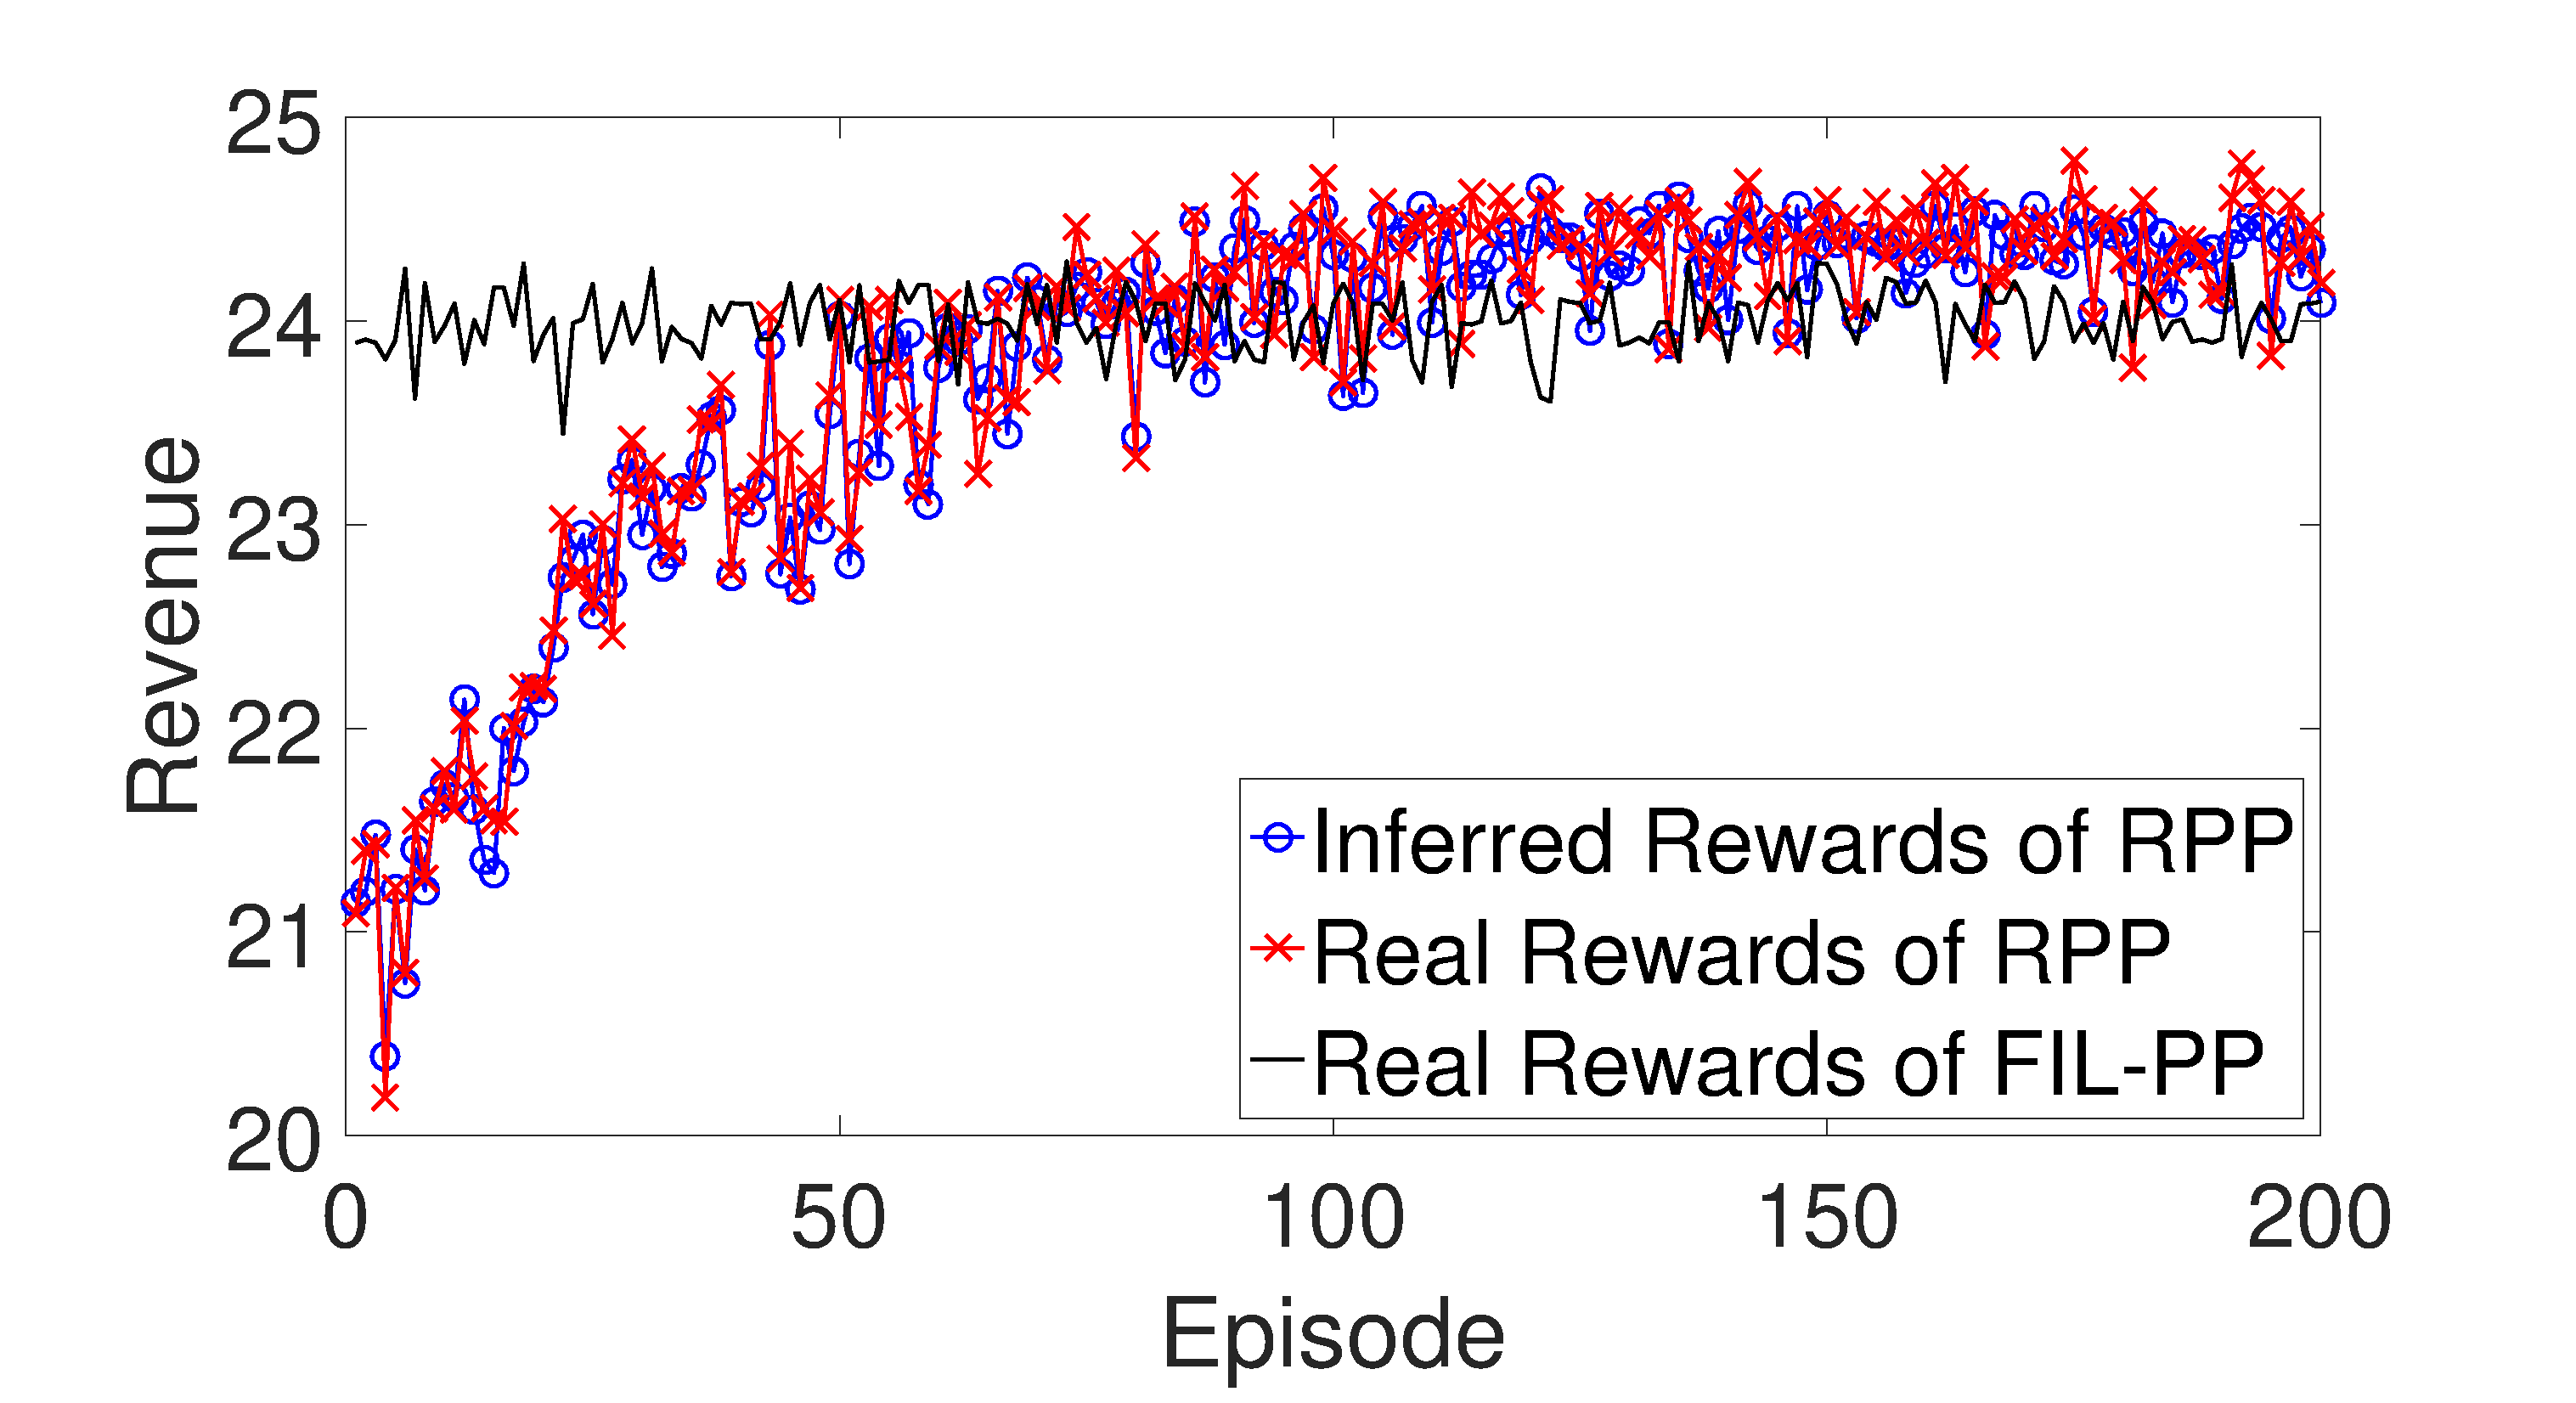
\includegraphics[width=\textwidth]{image/1}
        \caption{\label{E1} Fully Rational Workers}
    \end{subfigure}%
    ~\hspace{-6mm}
    \begin{subfigure}[t]{0.35\textwidth}
        \centering
        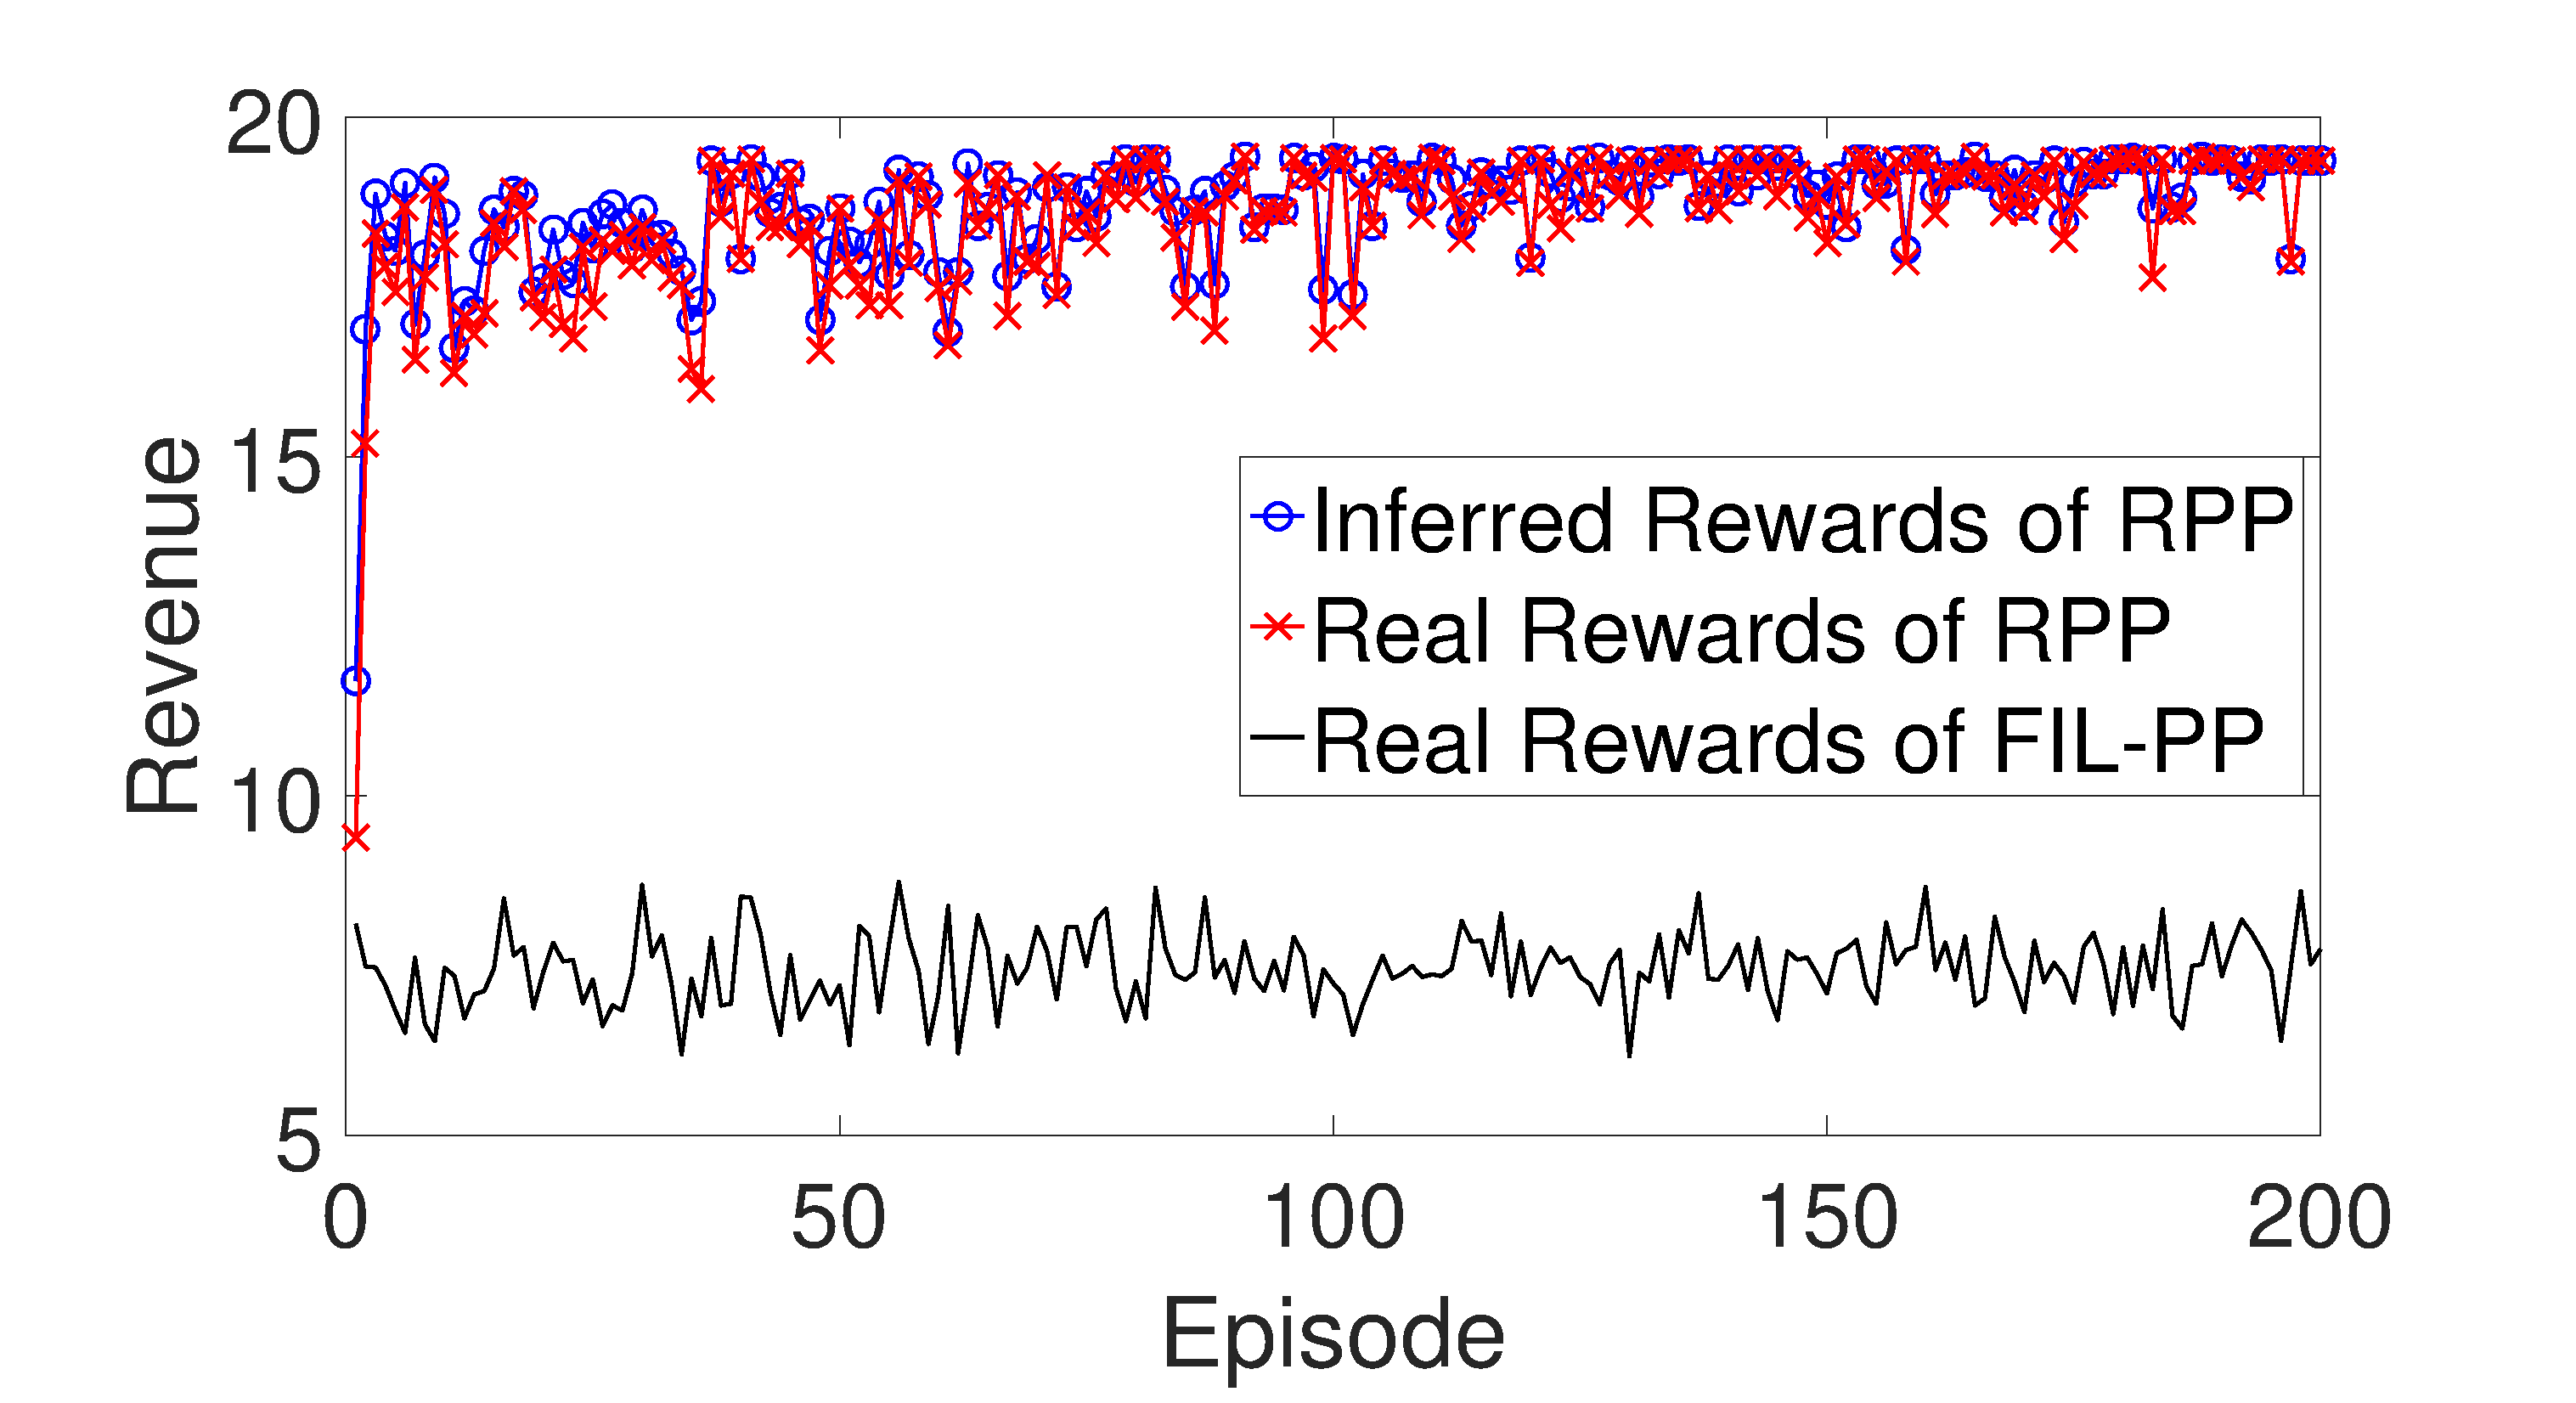
\includegraphics[width=\textwidth]{image/2}
        \caption{\label{E2}  Quantal Response Workers}
    \end{subfigure}
    ~\hspace{-8mm}
    \begin{subfigure}[t]{0.35\textwidth}
        \centering
        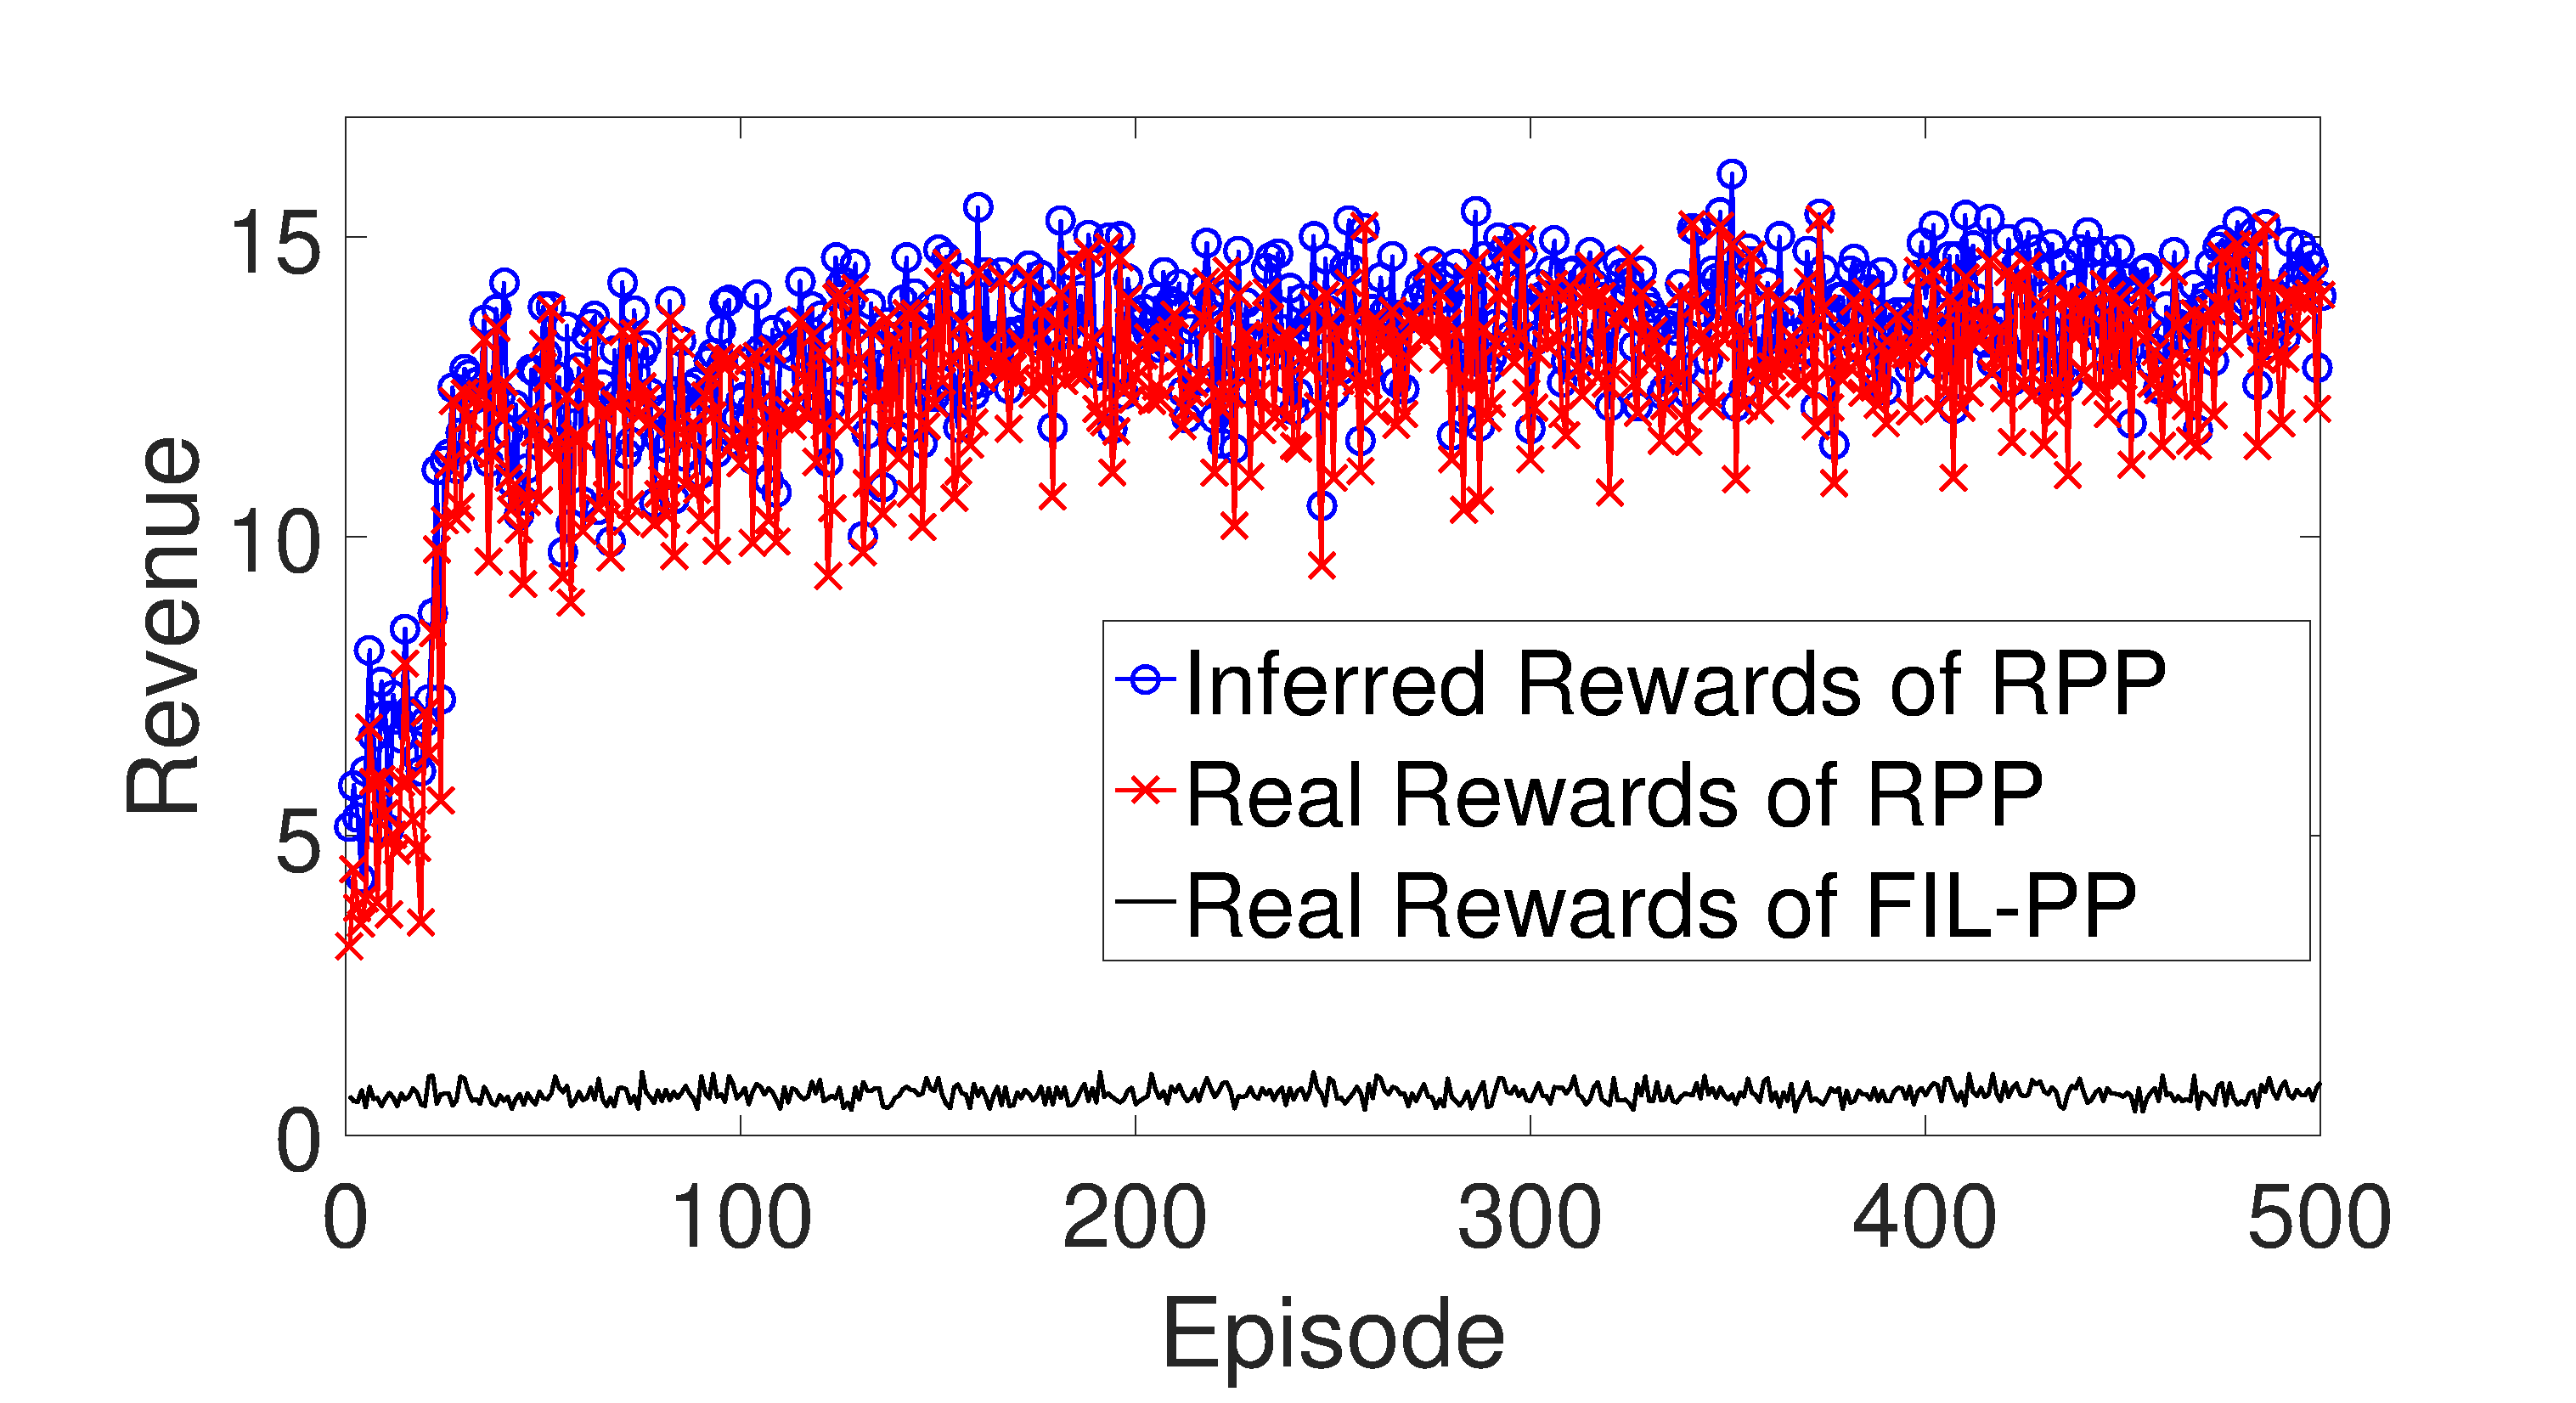
\includegraphics[width=\textwidth]{image/3}
        \caption{\label{E3}  MWU Workers}
    \end{subfigure}
    \caption{\label{ED}Experiments on three popular worker models}
\end{figure*}
\subsection{Reinforcement Learning} 
Recall that when computing the scaling level $I_{t}$ for step $t$, we do not observe workers' labels and thus cannot estimate the current state $s_{t}$ via Bayesian inference.
In this case, we cannot build the scaling level adjustment policy by directly using the the learned state of the whole workers.
Meanwhile, the number of labels the data requester collected at one time is usually very limited.
If there are still many unlabeled tasks remaining, the policy may tend to use high scaling levels to impress workers with the importance of high effort. On the other hand, if there are only few tasks left, we may prefer low scaling levels to reduce the payment.
Thus, our scaling level adjustment policy should take the number of unlabeled tasks into consideration.


To define our policy, we firstly introduce the augmented state of our mechanism as 
\begin{equation}
\hat{s}_t=\langle s_{t-1}, I_{t-1}, T-t \rangle.
\end{equation}
where $s_{t-1}$ and $I_{t-1}$ reflect the current state, and $T-t$ can denote the number of unlabeled tasks because we collect labels for a fixed number of tasks at each step.
Then, our task adjustment policy $\pi(I_{t}|\hat{s}_t)$.
Typically, in model-free reinforcement learning methods, $Q$-function, which calculates the expected reward of taking a given action in a given state and following the current policy afterwards, is heavily used to iteratively improve the adopted policy.
Putting into the context of our problem, the $Q$-function of our scaling level adjustment policy can be calculated as
\begin{equation}
Q(\hat{s}_t, I_t)= {\sum}_{i=0}^{T-t} \gamma^{i} r_{t+i}.
\end{equation}
Then, our policy can be formally written as
\begin{equation}
I_t = \arg\max_{I\in W} Q(\hat{s}_t, I_t).
\end{equation}

Another challenge of our mechanism is that both the state $s_t$ and reward $r_t$ can not be accurately observed.
Thus, we approximate the temporal difference (TD) by assuming that the residual follows a Gaussian process:
\begin{equation}
r_t\approx Q(\hat{s}_t, I_t) - \gamma Q(\hat{s}_{t+1}, I_{t+1}) + N(\hat{s}_t,\hat{s}_{t+1})
\end{equation}
where $N(\hat{s}_t,\hat{s}_{t+1})\sim \mathcal{N}(0, \sigma^2)$ approximates the residual.
Here, we use the Gaussian distribution to approximate the residual because of two reasons.
Firstly, the Gaussian distribution assumption greatly simplifies our derivation.
Secondly, our empirical results later show that this approximation has achieved robust performance under different worker models.

Under the Gaussian process approximation, we can put all the observed rewards and the corresponding $Q$-function up to the current step $t$ together and obtain
\begin{equation}
\bm{r}=\bm{H}\bm{Q}+\bm{N}
\end{equation}
where $\bm{r}$, $\bm{Q}$ and $\bm{N}$ denote the collection of rewards, $Q$ values, and residual values up to step $t$, respectively.
Due to the Gaussian process assumption of the residual, $\bm{N}\sim \mathcal{N}(\bm{0},\bm{\sigma}^2)$, where $\bm{\sigma}^2=\textrm{diag}(\sigma^2,\ldots,\sigma^2)$.
The hat matrix $\bm{H}$ satisfies that $\bm{H}(k,k)=1$ and $\bm{H}(k,k+1)=-\gamma$ for $k=1,\ldots, t$.
Then, the Q-function can be learned effectively using the online Gaussian process regression algorithm~\cite{engel2005reinforcement}. Furthermore, we use the classic $\epsilon$-greedy policy to learn the $Q$-function. More specifically,
\begin{itemize}
\item with a probability of $1-\epsilon$, $\arg\max_{I_t} Q(\hat{s}_{t}, I_{t})$ is chosen; 
\item with a probability of $\epsilon$, a random $I_t$ is set. 
\end{itemize}
We define an episode of our mechanism as employing workers to finish $T\cdot M$ tasks.
To reduce the effects of $\epsilon$, we set $\epsilon_{i+1}=(1-\sigma)\cdot \epsilon_{i}$, where the subscript $i$ denotes the number of episodes and $\sigma$ is a very small number.


\section{Experiments}

Figure~\ref{ED} shows our experimental results on three popular worker models.
Similar to the previous studies~\cite{liu2017sequential}, we assume that there are two effort levels, High and Low, that a worker can potentially choose from.
If a worker choose the high effort, it will report the correct label with probability $0.9$ (to capture a simple case with bounded rationality); otherwise, it will randomly report the label --- i.e. the probability of being correct is $0.5$.
Then, the three worker models can be described as
\begin{itemize}
\item \textbf{Rational Workers}: Since the peer prediction mechanism can theoretically ensure that exerting the maximal effort is the optimal action for all workers, we assume that rational workers will choose the high effort level, when scaling level is high enough to cover his cost.
\item \textbf{Quantal Response Workers}~\cite{mckelvey1995quantal}: The quantal response worker will choose the high level of effort with the following probability
\begin{equation}
\text{Pr}(H)= \frac{\exp (\lambda\cdot u_H)}{\exp (\lambda\cdot u_H)+\exp (\lambda\cdot u_L)}
\end{equation}
where $u_H$ and $u_L$ denote workers' expected utility of exerting high and low effort, respectively. $\lambda$ denotes workers' rationality level, and we set $\lambda=3$ in our experiments.
\item \textbf{MWU Workers}~\cite{chastain2014algorithms}: The multiplicative weight update (MWU)  workers uses a mixed strategy $[\text{Pr}_t(H), \text{Pr}_t(L)]$ to decide their effort levels at step $t$. After receiving the payment from our mechanism, they will update their strategy as
\begin{equation}
\begin{split}
\text{Pr}_{t+1}(H) = Z\cdot \text{Pr}_t(H)\cdot (1+\bar{u}_H)\\
\text{Pr}_{t+1}(L) =  Z\cdot \text{Pr}_t(L)\cdot (1+\bar{u}_L)
\end{split}
\end{equation}
where $Z$ is the normalizing constant used to maintain a valid probability measure. $\bar{u}_H$ and $\bar{u}_L$ are the average utility of high and low effort, respectively.
\end{itemize}
Note that we only model agents using existing bounded rationality models here. More sophisticated worker model, e.g. the forward-looking ones, will be studied in future work.

Furthermore, in our experiments, we assume there are four available scaling levels for our mechanism to choose, namely $I_t \in W=\{0.1, 1.0, 5.0, 10.0\}$.
In practice, traditional one-shot peer prediction mechanisms are often implemented with a fixed scaling level. Because of this, we set up a mechanism with a fixed scaling level of $1.0$ as baseline and we denote it as FIL-PP.
By contrast, our reinforcement peer prediction (RPP) mechanism can dynamically learn and adjust the scaling level to maximize data requester's revenue.
Based on all experiment results, we find that our mechanism is robust, and is able to significantly increase data requester's revenue, especially when workers are not fully rational.


Besides, in Figure~\ref{ED2}, we present the comparison of accuracy errors between the classic Dawid-Skene estimator~\cite{dawid1979maximum} and our Gibbs sampling estimator.
The results show that our estimator can significantly reduce the errors of $A_t$ and $F(A_t)$ estimations.
More accurate estimation of $F(A_t)$ provides a higher quality reward signal, which warrants the good performance of our closed-loop reinforcement framework.


\begin{figure}[htb]
    \hspace{-8mm}
     \includegraphics[width=0.55\textwidth]{image/4}
    \caption{\label{ED2} Mean errors of accuracy estimations in 200 runs}
\end{figure}

\section{Conclusions and Future Work}
In this paper, we propose a novel reinforcement peer prediction mechanism.
It maximizes the revenue of the data requester by dynamically adjusting the scaling level of a peer prediction payment function based on workers' labels.
Compared with existing peer prediction mechanisms, our mechanism does not require to assume a decision-making model for workers and uninformative equilibrium where agents report uninformative information is a bad equilibrium.
To achieve above, we firstly develop a Bayesian inference algorithm to evaluate workers' contributions, and to infer the reward following each offered scaling level. 
Then, we learn the optimal scaling level adjustment strategy by approximating the $Q$-function of our mechanism with the Gaussian process.
We conduct empirical evaluation on three popular worker models, and the results show that our mechanism is robust, and is able to significantly increase data requester's revenue.

In future, we wish to improve our mechanism in the following two aspects.
Firstly, more complex worker models and actions should be considered.
To the best of our knowledge, this paper is the first work to adjust the peer prediction mechanism based workers' labels.
In this case, except for the existing bounded rationality models, we cannot find models that characterize workers' more complex behaviors, e.g. forward-looking.
Meanwhile, our interaction with workers is limited to the scaling level, while the practical crowdsouricng platform can affect workers by, for example, sending them an alert or forcing them to take a training step.
Currently, we can not find proper models for workers' response to these actions.
Secondly, we can improve the convergence speed of our reinforcement learning algorithm by introducing more complex learning structures, for example, the actor-critic algorithm.
Besides, we also consider to build a deep reinforcement peer prediction mechanism which directly uses the collected labels as the state.
By doing so, we can avoid using the Bayesian inference algorithm which assumes a fixed confusion matrix for one worker.

\section*{Acknowledgments}
This work was conducted within Rolls-Royce@NTU Corporate Lab
with support from the National Research Foundation (NRF) Singapore
under the Corp Lab@University Scheme. The authors also thank Anxiang Zeng from Alibaba Group for valuable discussions.

\bibliographystyle{aaai}
\bibliography{ref}

\end{document}
